
\section{Introduction}

	\defn{Web Application}{is a distributed information management system. In
essence it is an application , usually spread around several machines, which allows
users to query and manipulate data, and which is then displayed via the browser}

	\rem{The distinction between a website and a web app is less clear nowadays,
but the main feature of a web app seems to be its interactive nature, as opposed
to the more expository nature of simple websites}

	\defn{Distributed Information Management System (DIM)}{a
group of machines working together but appearing to the user as a single entity.
These systems have major advantages, such as concurrent and independent
operation. One machine can fail or be upgraded without the system failing}

\subsubsection{Architecture}
	
	\par{A common system architecture for a DIM is represented in the diagram
below. Web development has a wide range of tools and new frameworks and
languages come into being every other week. In this class, we'll focus on the
tools listed below but in general each tool group performs certain tasks which
are essential to each bit of the system}

	\rem{Most web apps follow a 3-tier architecture : Presentation, Application,
			Data. The rango app will also include an external service , the Bing
	search API}

	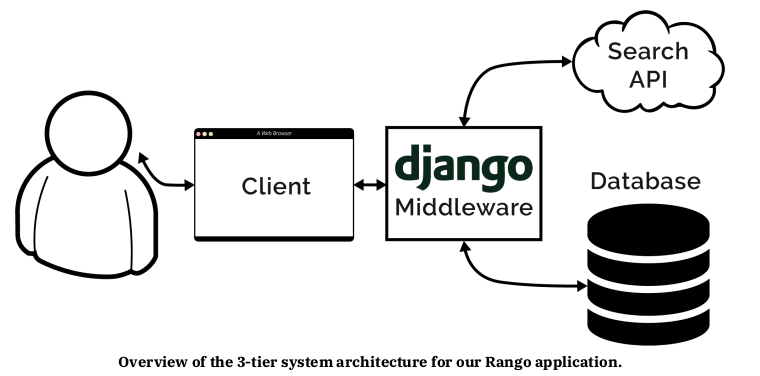
\includegraphics[width=\textwidth]{3arch}
	\defn{User}{machine or person which initiates contact with the client}

	\defn{Client}{program sitting on the user device which sends/accepts
requests/responses and acts on the messages by communicating to them the user
and/or by altering state in some way}

	\rem{A request is usually done via \texttt{HTTP} where the data to be sent is
	embedded, and responses are also sent via \texttt{HTTP} with content usually
	delivered in a markup language like \texttt{XHTML} or \texttt{JSON}}

	\defn{Middleware}{Responsible for accepting and sending responses on server
side and for coordinating messages}

	\rem{In this course we'll be using Django}

	\rem{The database is usually kept in a separate node}

\subsubsection{Tools Covered}
	
		\mymarginpar{Proficiency expected}
		\begin{multicols}{2} 
				\begin{enumerate}
					\item Python
					\item Django
					\item HTML/CSS
					\item HTTP GET/POST
					\item XML/XHTML/JSON
					\item JS
					\item JQuery
					\item AJAX
					\item Github
					\item Pip
					\item PythonAywhere
					\item IDLE
					\item Venv
					\item Draw.io
				\end{enumerate}
		\end{multicols}

\end{document}
